\paragraph{QuizziPedia::Back-End::App::Models::UserModel}
\label{QuizziPedia::Back-End::App::Models::UserModel}
\begin{figure}
	\centering
	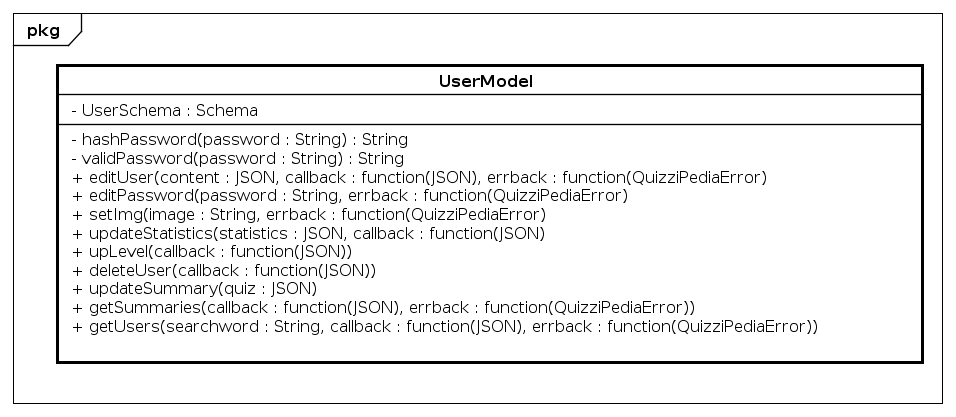
\includegraphics[scale=0.45]{UML/Package/QuizziPedia_Back-End_App_Models_userModel.png}
	\caption{QuizziPedia::Back-End::App::Models::UserModel}
\end{figure}
\begin{itemize}
	\item \textbf{Descrizione} \\
	Classe che modella la creazione e la gestione dei dati utente
	\item \textbf{Utilizzo} \\
	Viene utilizzata per rappresentare i dati degli account dei vari utenti dell'applicazione. Si interfaccia alla libreria Mongoose per la creazione dello schema e dei relativi metodi statici o di istanza.
	\item \textbf{Relazioni con altre classi} 
		\begin{itemize}
			\item \textbf{IN SummaryModel} \\
			Questa classe rappresenta il riepologo dei questionari svolti dagli utenti.
			\item \textbf{OUT QuestionModel} \\
			Questa classe rappresenta i dati delle domande create dai vari utenti.
			\item \textbf{OUT QuizModel} \\
			Questa classe rappresenta i dati dei questionari creati dagli utenti Pro.
			\item \textbf{OUT UserProModel} \\
			Questa classe rappresenta i dati riguardanti l'utente pro.
		\end{itemize}
	\item \textbf{Attributi} 
		\begin{itemize}
			\item \textbf{- \texttt{userSchema}: \texttt{Schema}} \\
			Questo campo dati rappresenta lo schema Mongoose dell'utente QuizziPedia. Lo schema prevede i seguenti attributi:
			\begin{itemize}
				\item 
					\texttt{name} di tipo \texttt{String}, rappresenta il nome  dell'utente registrato;
				\item 
					\texttt{surname} di tipo \texttt{String}, rappresenta il cognome  dell'utente registrato;
				\item 
					\texttt{email} di tipo \texttt{String}, rappresenta l'email  dell'utente registrato;
				\item 
					\texttt{userImg} di tipo \texttt{String}, rappresenta il path della foto profilo dell'utente registrato;
				\item 
					\texttt{username} di tipo \texttt{String}, rappresenta l'username con cui viene identificato l'utente all'interno dell'applicazione;		
				\item
					\texttt{password} di tipo \texttt{String}, rappresenta la password associata all'utente,  appositamente codificata mediante l'algoritmo bcrypt;  		
				\item
					\texttt{statistics} di tipo \texttt{Array Mixed}, contenente i seguenti attributi:
				\begin{itemize}
					\item
						\texttt{topicName} di tipo \texttt{String}, rappresenta il nome della statistica relativa all'argomento;	 
					\item
						 \texttt{topicLevel} di tipo \texttt{Number}, identifica il livello di preparazione dell'utente in un determinato argomento;
					\item
						\texttt{correctAnswers} di tipo \texttt{Number}, identifica il numero di risposte corrette date dall'utente riguardanti domande di un determinato argomento; 
					\item						
						 \texttt{totalAnswers} di tipo \texttt{Number} , identifica il numero di risposte totali date dall'utente riguardanti domande di un determinato argomento.		
				\end{itemize}		
				\item 
					\texttt{levelUsers} di tipo \texttt{Number}, identifica il livello dell'utente;				
				
				\item
					\texttt{quizSummaries} di tipo \texttt{Array}, contiene oggetti di tipo \texttt{ObjectId}, che rappresentano i riferimenti agli identificativi nel database dei questionari svolti dall'utente;		
			\end{itemize}	
		\end{itemize}	
	\item \textbf{Metodi}
		\begin{itemize}
		\item
		- \texttt{generateHash(password: String): String} \\
		Effettua l'hashing della stringa password se non è già stata criptata tramite campo salt per evitare attacchi di tipo rainbow. \\
		\textbf{Parametri} 
			\begin{itemize}
			\item
				 \texttt{password: String} \\
				Rappresenta la password dell'utente.
			\end{itemize}
		\item
		- \texttt{validPassword(password: String): String} \\
		Effettua la validità della password inserita comparandola con la password criptata.	\\
		\textbf{Parametri} 
			\begin{itemize}
			\item
				\texttt{password: String} \\
				Rappresenta la password dell'utente.
			\end{itemize}
		\end{itemize}	
\end{itemize}